\documentclass{article}%
\usepackage{amsmath}%
\usepackage{amsfonts}%
\usepackage{amssymb}%
\usepackage{graphicx}
\usepackage{enumitem}
%-------------------------------------------
\newtheorem{theorem}{Theorem}
\newtheorem{acknowledgement}[theorem]{Acknowledgement}
\newtheorem{algorithm}[theorem]{Algorithm}
\newtheorem{axiom}[theorem]{Axiom}
\newtheorem{case}[theorem]{Case}
\newtheorem{claim}[theorem]{Claim}
\newtheorem{conclusion}[theorem]{Conclusion}
\newtheorem{condition}[theorem]{Condition}
\newtheorem{conjecture}[theorem]{Conjecture}
\newtheorem{corollary}[theorem]{Corollary}
\newtheorem{criterion}[theorem]{Criterion}
\newtheorem{definition}[theorem]{Definition}
\newtheorem{example}[theorem]{Example}
\newtheorem{exercise}[theorem]{Exercise}
\newtheorem{lemma}[theorem]{Lemma}
\newtheorem{notation}[theorem]{Notation}
\newtheorem{problem}[theorem]{Problem}
\newtheorem{proposition}[theorem]{Proposition}
\newtheorem{remark}[theorem]{Remark}
\newtheorem{solution}[theorem]{Solution}
\newtheorem{summary}[theorem]{Summary}
\newcommand\abs[1]{\left|#1\right|}
\newcommand\EXP[1]{\exp\left(#1\right)}
\newcommand\Res[1]{\text{Res}{#1}}
\newcommand\I{\textbf{i}}
\newenvironment{proof}[1][]{\textbf{Proof #1} \\ }{\\ \rule{0.5em}{0.5em}  \\}
\setlength{\textwidth}{7.0in}
\setlength{\oddsidemargin}{-0.35in}
\setlength{\topmargin}{-0.5in}
\setlength{\textheight}{9.0in}
\setlength{\parindent}{0.3in}
\begin{document}

\begin{flushright}
\textbf{Brandon Toner \\
\today}
\end{flushright}

\begin{center}
\textbf{MATH 438: Introduction to Complex Variables \\
Final Exam} \\
\end{center}

\begin{enumerate}
    \item %1
    \begin{enumerate}[label=\alph*)]
        \item %1.a
        \textbf{State Green's Theorem for a multiply-connected domain $D$ and draw a picture:}
        \begin{eqnarray*}
            \int\limits_{\partial D} u~dx+ v~dy &=& \int\int\limits_{D} v_x - u_y~dx~dy
        \end{eqnarray*}
        \begin{center}
            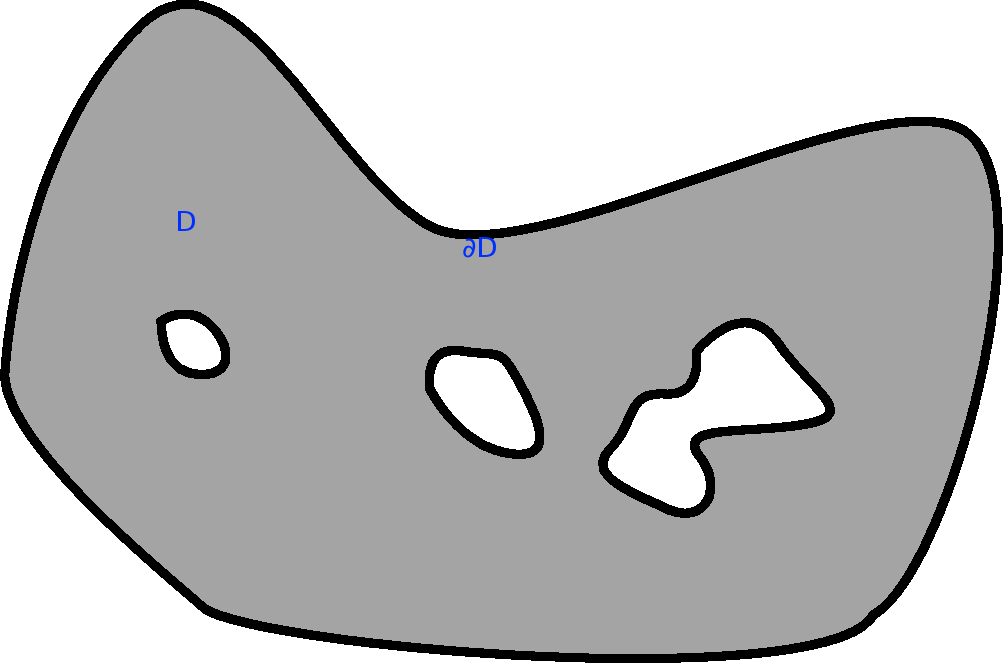
\includegraphics[width=\textwidth]{images/greens.png}
        \end{center}
        \item %1.b
        \textbf{Using Green's Theorem for a multiply-connected domain $D$, prove the Deformation Theorem for $f$ analytic on $D \cup \partial D$.} \\
        \textbf{Theorem: } Let $f(z)$ be analytic on domain $D \cup \partial D$, bounded by $\Gamma \cup \gamma_1 \cup ... \cup \gamma_n$. Then
        \begin{eqnarray*}
            \int\limits_{\Gamma}{f(z)~dz} &=& \sum\limits_{n=1}^k \int\limits_{\gamma_n}{f(z)~dz} \\
        \end{eqnarray*}
        \begin{proof}
            Assume $\gamma_1, ..., \gamma_k$ are ordered such that $\gamma_n$ and $\gamma_{n+1}$ can be connected with a line segment that does not
            intersect any other $\gamma_j$. Draw line segments $\Phi_0, ..., \Phi_k$ such that for $1\leq n\leq k-1$, $\Phi_n$ connects $\gamma_n$ and
            $\gamma_{n+1}$. $\Phi_0$ and $\Phi_k$ connect $\Gamma$ to $\gamma_1$ and $\gamma_k$. $D$ is now divided into two simply connected domains,
             $D_1$ and $D_2$, by $\Gamma \cup \gamma_1 \cup ... \cup \gamma_k \cup \Phi_0 \cup ... \cup \Phi_k$. Now, by Cauchy's Theorm, 
            \begin{eqnarray*}
                \int\limits_{\partial D_1}f(z)~dz &=& 0 \\
                \int\limits_{\partial D_2}f(z)~dz &=& 0 \\
                \int\limits_{\partial D_1 \cup \partial D_2}{f(z)~dz} &=& 0 \\
            \end{eqnarray*}
            Since $\Phi_0, ..., \Phi_k$ were traversed in opposite directions in $\partial D_1$ and $\partial D_2$
            \begin{eqnarray*}
                \int\limits_{\partial D}{f(z)~dz} &=& 0 \\
                \int\limits_{\Gamma\cup\gamma_1 \cup ... \cup \gamma_k}{f(z)~dz} &=& 0 \\
                \int\limits_{\Gamma}{f(z)~dz} + \int\limits_{\gamma_1 \cup ... \cup \gamma_k}{f(z)~dz} &=& 0 \\
                \int\limits_{\Gamma}{f(z)~dz} + \sum\limits_{n=1}^k{\int\limits_{\gamma_n}{f(z)~dz}} &=& 0 \\ 
            \end{eqnarray*}
            $\gamma_n$ is currently being traversed in the opposite direction of $\Gamma$, but if we let $\hat{\gamma_n}$ be $\gamma_n$ traversed in the
            same direction as $\Gamma$,
            \begin{eqnarray*}
                \int\limits_{\Gamma}{f(z)~dz} &-& \sum\limits_{n=1}^k{\int\limits_{\hat{\gamma_n}}{f(z)~dz}} = 0 \\
                \int\limits_{\Gamma}{f(z)~dz} &=& \sum\limits_{n=1}^k{\int\limits_{\hat{\gamma_n}}{f(z)~dz}} \\
            \end{eqnarray*}
        \end{proof}
        \item %1.c
        \textbf{Complete: For $f(z)$ be analytic on $D\cup\partial D$, the Cauchy integral formula says} \\
        \begin{eqnarray*}
            f(z) &=& \frac{1}{2\pi\I} \int\limits_{\gamma}{\frac{f(\xi)}{\xi - z} d\xi} ~~\forall z \text{ inside } \gamma
        \end{eqnarray*}
        \item %1.d
        \textbf{The Cauchy integral formula for derivatives says}
        \begin{eqnarray*}
            f^{(k)}(z) &=& \frac{k!}{2\pi\I}\int\limits_{\gamma}{\frac{f(\xi)}{(\xi - z)^{k+1}} d\xi} ~~\forall z \text{ inside } \gamma
        \end{eqnarray*}
        \item %1.e
        \textbf{Prove the Cauchy integral formula for derivatives.} \\
        \begin{proof}[by induction]
            Base case: $k = 1$\\
            Let $z$ be any value inside $\gamma$. From the Cauchy integral formula, we know
            \begin{eqnarray*}
                f(z) &=& \frac{1}{2\pi\I} \int\limits_{\gamma}{\frac{f(\xi)}{\xi - z} d\xi} \\
                f^{(1)}(z) &=& \frac{d}{dz}\left[\frac{1}{2\pi\I} \int\limits_{\gamma}{\frac{f(\xi)}{\xi - z} d\xi}\right] \\
                           &=& \frac{1}{2\pi\I}\int\limits_{\gamma}{\frac{f(\xi)}{(\xi - z)^2} d\xi}
            \end{eqnarray*}
            For $k\geq2$:
            \begin{eqnarray*}
                f^{(k)}(z) &=& \frac{k!}{2\pi\I}\int\limits_{\gamma}{\frac{f(\xi)}{(\xi - z)^{k+1}} d\xi} \\
                \frac{d}{dz} f^{(k)}(z) &=& \frac{d}{dz}\left[\frac{k!}{2\pi\I}\int\limits_{\gamma}{\frac{f(\xi)}{(\xi - z)^{k+1}} d\xi} \right]\\
                f^{(k+1)}(z) &=& \frac{k!}{2\pi\I}\int\limits_{\gamma}{\frac{d}{dz}\left[\frac{f(\xi)}{(\xi - z)^{k+1}} d\xi \right]} \\
                           &=& \frac{k!}{2\pi\I}\int\limits_{\gamma}{(k+1)\frac{f(\xi)}{(\xi - z)^{k+2}} d\xi} \\
                           &=& \frac{(k+1)!}{2\pi\I}\int\limits_{\gamma}{\frac{f(\xi)}{(\xi - z)^{(k+1)+1}} d\xi} \\
            \end{eqnarray*}
        \end{proof}
    \end{enumerate}
    \item %2
    \textbf{Find all the following integrals around the unit circle $\gamma$ using the Cauchy formulas}
    \begin{enumerate}[label=\alph*)]
        \item %2.a
        \begin{eqnarray*}
            \int\limits_{\gamma} \frac{z^3}{(2z-1)^2} dz &=& \int\limits_{\gamma}{\frac{\xi^3}{(2\xi-1)^2} d\xi} \\
                &=& \frac{1}{4}\int\limits_{\gamma}{ \frac{\xi^3}{(\xi-0.5)^2} d\xi} \\
                &=& \frac{2\pi\I}{4} \frac{1}{2\pi\I} \int\limits_{\gamma}{ \frac{\xi^3}{(\xi-0.5)^2} d\xi} \\
                &=& \frac{2\pi\I}{4} \left. \frac{d \xi^3}{d\xi} \right|_{\xi=0.5} \\
                &=& \frac{3\pi\I}{8}
        \end{eqnarray*}
        \item %2.b
        \begin{eqnarray*}
            \int\limits_{\gamma}{\frac{e^{2z}}{z^3}dz} &=& \int\limits_{\gamma}{\frac{e^{2\xi}}{\xi^3}d\xi}\\
                &=& \frac{2\pi\I}{2!} \left.\frac{d^2e^{2\xi}}{d\xi^2} \right|_{\xi=0} \\
                &=& 4\pi\I
        \end{eqnarray*}
        \item %2.c
        \begin{eqnarray*}
            \frac{1}{2\pi\I} \int\limits_{\gamma}{\frac{\cos(2z)}{z-0.5}dz} &=& \frac{1}{2\pi\I} \int\limits_{\gamma}{\frac{\cos(2\xi)}{\xi-0.5}d\xi} \\
                &=& \left. \cos(2\xi) \right|_{\xi=0.5} \\
                &=& \cos(1) \approx 0.540302
        \end{eqnarray*}
        \item %2.d
        Since $\frac{\cos(2z)}{z-2}$ is analytic on the simply connected domain bounded by $\gamma$,
        \begin{eqnarray*}
            \frac{1}{2\pi\I} \int\limits_{\gamma}{\frac{\cos(2z)}{z-2}dz} &=& 0\\
        \end{eqnarray*}
        by the Cauchy Theorem.
    \end{enumerate}
    \item %3
    \begin{enumerate}[label=\alph*)]
        \item %3.a
        \textbf{Explain what $O(z^m)$ stands for in the Taylor expansion of $f(z)$ centered at $0$} \\
        \begin{eqnarray*}
            f(z) &=& \sum\limits_{k=0}^{\infty}\frac{f^{(k)}(0)}{k!} z^k = \sum\limits_{k=0}^{m-1}\frac{f^{(k)}(0)}{k!} z^k + O(z^m)
        \end{eqnarray*}
        The $O(z^m)$ in the Taylor expansion of $f(z)$ centered at $0$ means the sum of the remaining terms is less than $c z^m$ for some $c>0$.
        \item %3.b
        \textbf{What would you insert in the following expression to make it complete?}
        \begin{eqnarray*}
            \frac{1}{1-z} &=& 1 + z + z^2 + O(z^3) \\
        \end{eqnarray*}
        \item %3.c
        \textbf{If $f(z)=a_0+a_1z+a_2z^2+O(z^3)$ and $g(z)=b_0+b_1z+b_2z^2+O(z^3)$ then complete the statement}
        \begin{eqnarray*}
            f(z)g(z) &=& a_0b_0+(a_0b_1+a_1b_0)z + (a_0b_2+a_1b_1+a_2b_0)z^2 + O(z^3)\\
        \end{eqnarray*}
        \item %3.d
        \textbf{If $f(z) = \sum\limits_{n=0}^{\infty}{a_nz^n}$ how would you write $O(z^3)$ (for $f$) in summation notation?}
        \begin{eqnarray*}
            f(z) = \sum\limits_{n=0}^{\infty}{a_nz^n} &=& \sum\limits_{n=0}^{2}{a_nz^n} + O(z^3) \\
                   \sum\limits_{n=3}^{\infty}{a_nz^n} &=& O(z^3)
        \end{eqnarray*}
    \end{enumerate}
    \item %4
    \textbf{Calculate the terms through order seven of the power series expansion about $z = 0$ of the function $1/\cos(z)$.}\\
    \begin{align*}
        f^{(0)}(0) &                                                                                                                    &= 1 \\
        f^{(1)}(0) &= \left. \frac{df^{(0)}(z)}{dz}\right|_{z=0} = \frac{\sin(0)}{\cos^2(0)}                                            &= 0 \\
        f^{(2)}(0) &= \left. \frac{df^{(1)}(z)}{dz}\right|_{z=0} = \frac{\sin^2(0)+1}{\cos^3(0)}                                        &= 1 \\
        f^{(3)}(0) &= \left. \frac{df^{(2)}(z)}{dz}\right|_{z=0} = \frac{\sin(0)(\sin^2(0)+5)}{\cos^4(0)}                               &= 0 \\
        f^{(4)}(0) &= \left. \frac{df^{(3)}(z)}{dz}\right|_{z=0} = \frac{\sin^2(0)(\sin^2(0)+18)+5}{\cos^5(0)}                          &= 5 \\ 
        f^{(5)}(0) &= \left. \frac{df^{(4)}(z)}{dz}\right|_{z=0} = \frac{\sin(0)(\sin^4(0)+58\sin^2(0)+61)}{\cos^6(0)}                  &= 0 \\
        f^{(6)}(0) &= \left. \frac{df^{(5)}(z)}{dz}\right|_{z=0} = \frac{\sin^6(0)+179\sin^4(0)+478\sin^2(0)+61}{\cos^7(z)}             &= 61 \\
        f^{(7)}(0) &= \left. \frac{df^{(6)}(z)}{dz}\right|_{z=0} = \frac{\sin(0)(\sin^6(0)+543\sin^4(0)+3111\sin^2(0)+1385)}{\cos^8(0)} &= 0 \\
        f(z)       &= 1 + \frac{z^2}{2} + \frac{5 z^4}{24} + \frac{61 z^6}{720} + O(z^8) 
    \end{align*}
    \item %5
    \textbf{Let $\overline{f(z)}$ be a velocity field of a fluid flowing over a domain $D$ and let $\gamma$ be a curve in $D$.}
    \begin{enumerate}[label=\alph*)]
        \item %5.a
        \textbf{State a formula for the circulation and flow rate of $\overline{f(z)}$ along and across $\gamma$ in terms of a complex integral.}
        \begin{eqnarray*}
            \text{Flow rate along $\gamma$ } &=& \int\limits_{\gamma}{\overline{f(z)}\cdot dz}\\
            \text{Flow rate across $\gamma$ } &=& \int\limits_{\gamma}{\overline{f(z)}\cdot -\I~dz}
        \end{eqnarray*}
        \item %5.b
        \textbf{Graph the velocity vector field $\overline{f(z)}$ for $f(z)=\frac{1}{z}$ and find its circulation and flux along and across the unit circle.}
        \begin{center}
            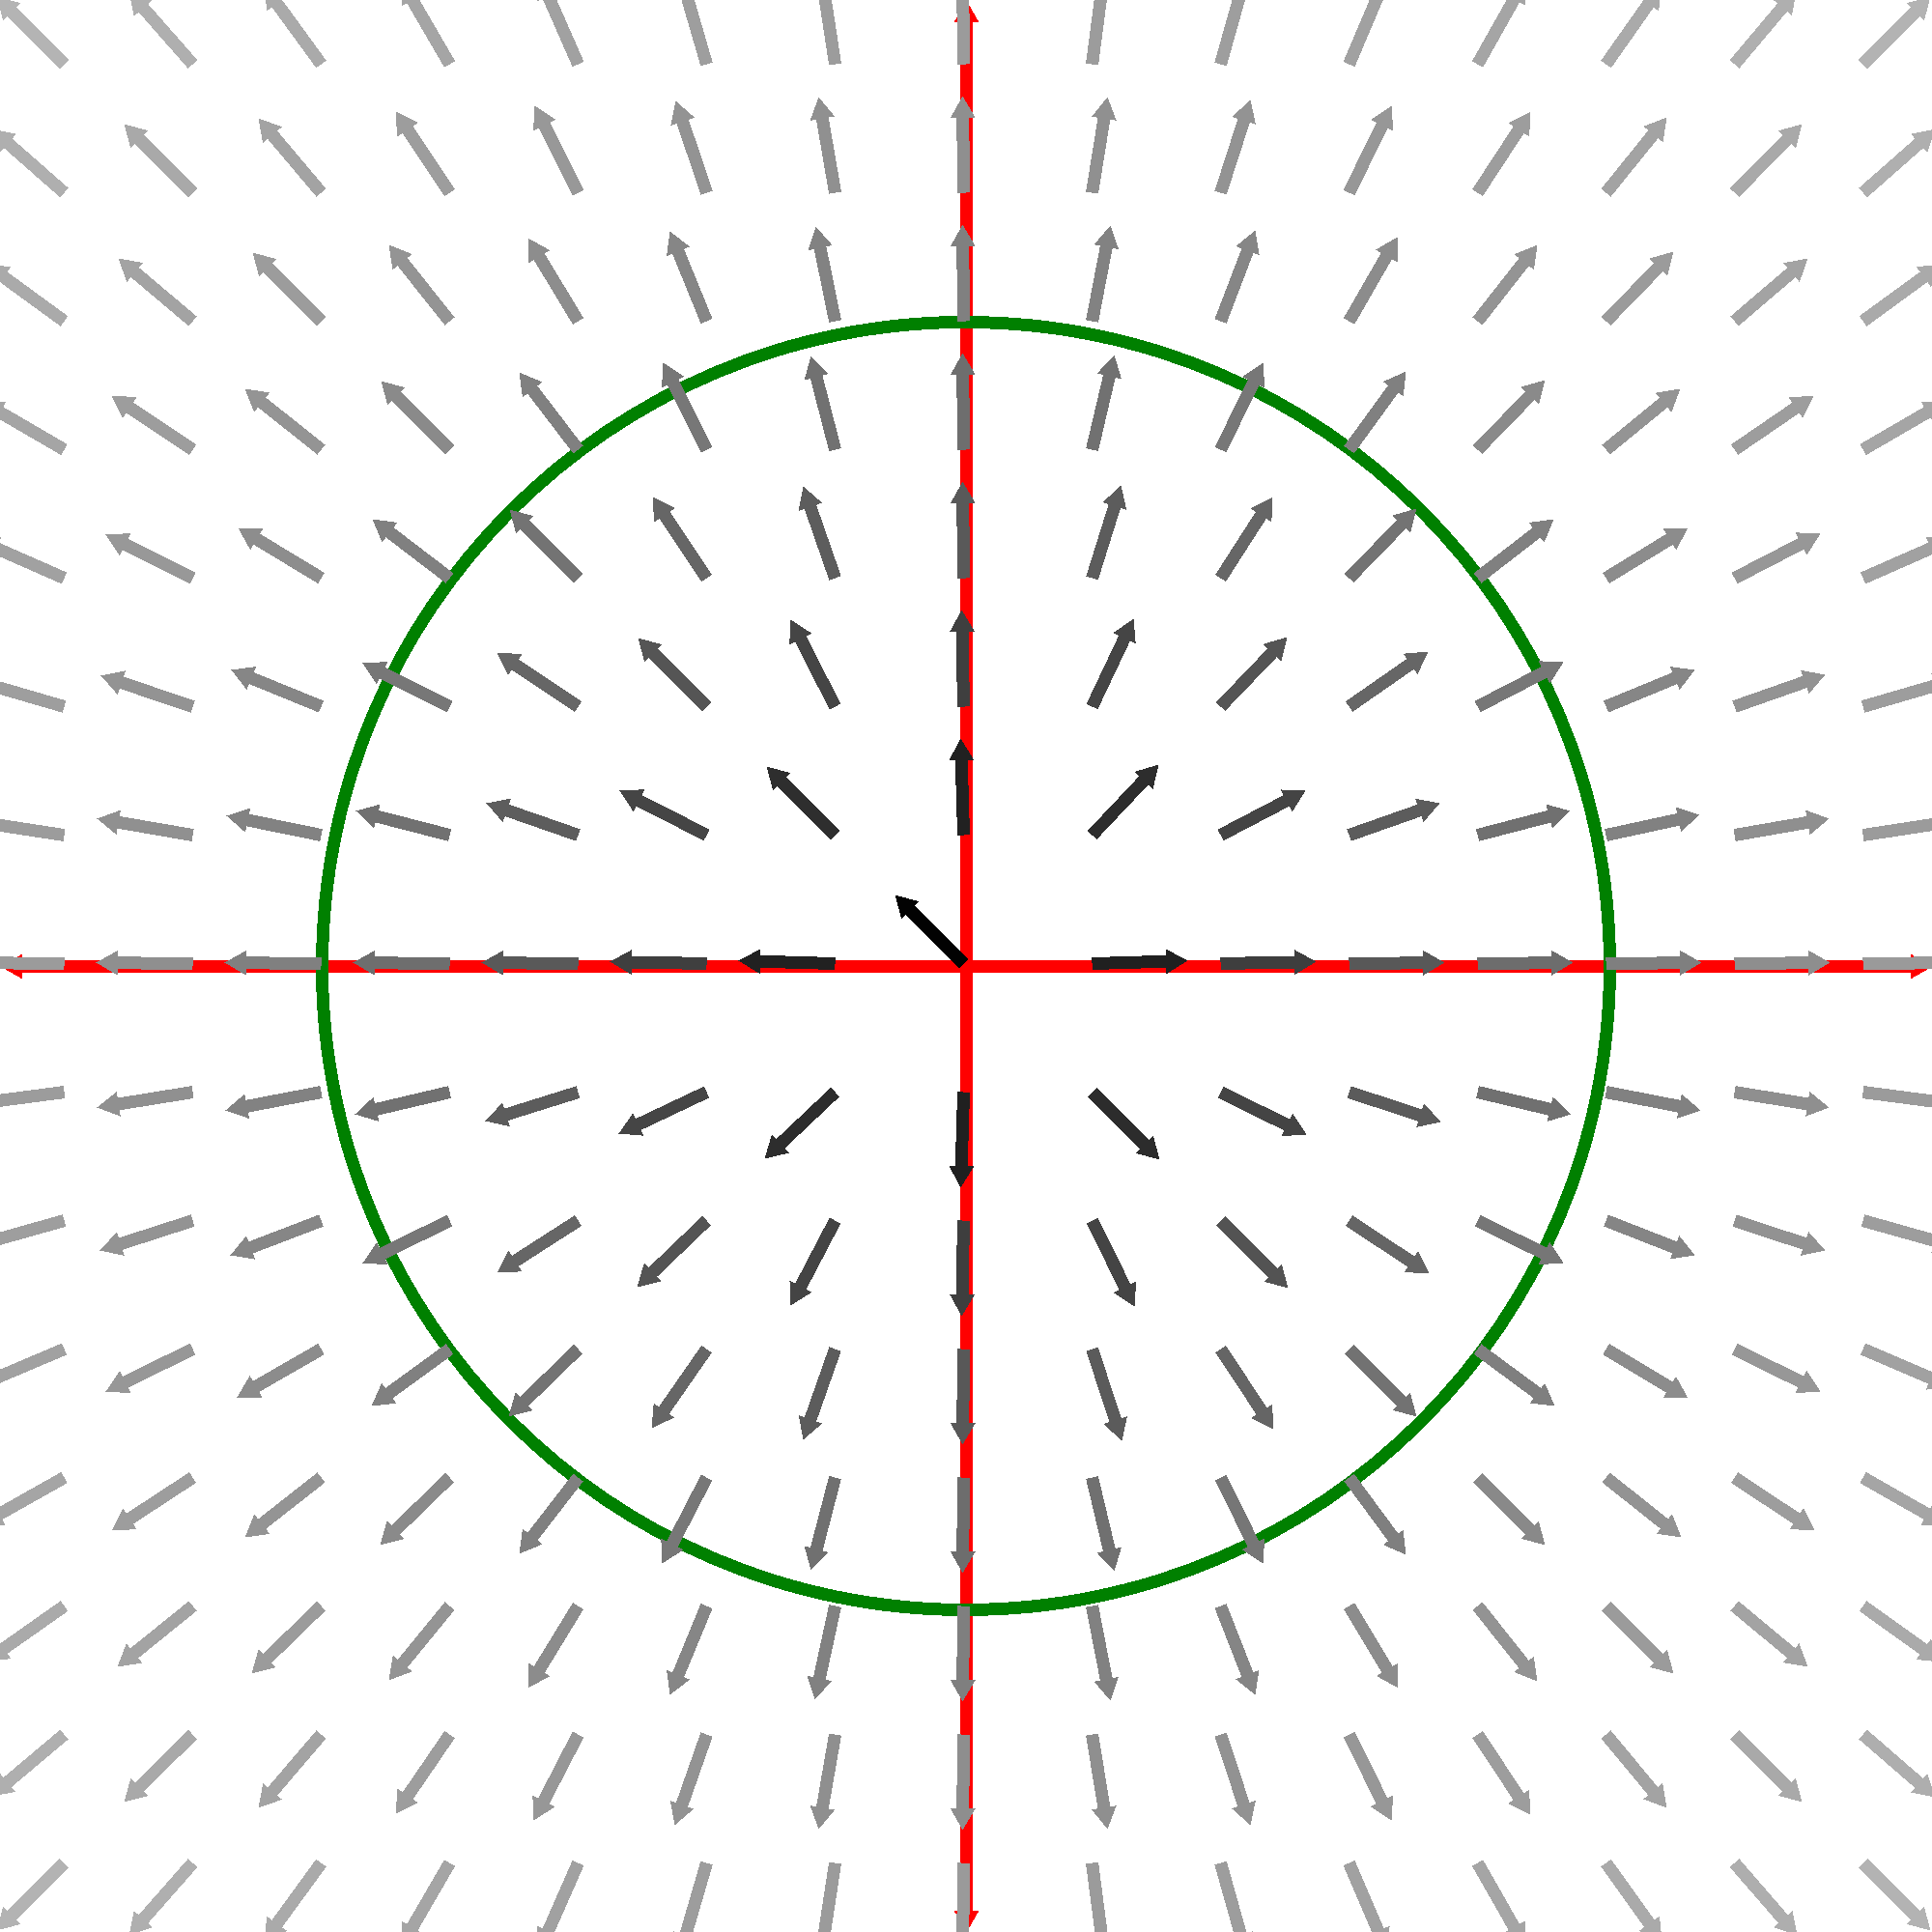
\includegraphics[scale=0.2]{images/z_inverse_conj.png} \\
            Green circle is the unit circle. Arrows point in direction of $\overline{f(z)}$, and get darker as $\abs{\overline{f(z})}\to\infty$
        \end{center}
        \begin{eqnarray*}
            \text{Flow rate along $\gamma$ } &=& \int\limits_{\gamma}{\overline{f(z)}\cdot dz} \\
                &=& \int\limits_{\gamma}{\overline{\left(\frac{1}{z}\right)}\cdot dz} \\
                &=& \int\limits_{\gamma}{\overline{\left(\frac{\bar{z}}{z\bar{z}}\right)} \cdot dz} = \int\limits_{\gamma}{\frac{z}{\abs{z}^2} \cdot dz} \\
                &=& \int\limits_{0}^{2\pi}{\frac{\cos(\theta)+\I\sin(\theta)}{1} \cdot (-\sin(\theta)+\I\cos(\theta)) d\theta} \\
                &=& \int\limits_{0}^{2\pi}{-\cos(\theta)\sin(\theta)+\sin(\theta)\cos(\theta) d\theta} = \int\limits_{0}^{2\pi}{0~d\theta} \\
                &=& 0
        \end{eqnarray*}
        \begin{eqnarray*}
            \text{Flow rate across $\gamma$ } &=& \int\limits_{\gamma}{\overline{f(z)}\cdot -\I dz} \\
                &=& \int\limits_{\gamma}{\frac{z}{\abs{z}^2} \cdot -\I dz} \\
                &=& \int\limits_{0}^{2\pi}{\frac{\cos(\theta)+\I\sin(\theta)}{1} \cdot -\I(-\sin(\theta)+\I\cos(\theta)) d\theta} \\
                &=& \int\limits_{0}^{2\pi}{(\cos(\theta)+\I\sin(\theta)) \cdot (\cos(\theta)+\I\sin(\theta))d\theta} \\
                &=& \int\limits_{0}^{2\pi}{\cos^2(\theta) + \sin^2(\theta) d\theta} = \int\limits_{0}^{2\pi}{1~d\theta} \\
                &=& 2\pi
        \end{eqnarray*}
    \end{enumerate}
    \item %6
    \textbf{Find the Laurent expansions of $\frac{1}{z^2-z}$ centered at 0}
    \begin{eqnarray*}
        a_n &=& \frac{1}{2\pi\I}\int\limits_{C}{\frac{1}{(\xi-1)\xi^{n+1}}-\frac{1}{\xi^{n+2}}d\xi} \\
            &=& \frac{1}{2\pi\I}\int\limits_{C}{\frac{1}{(\xi-1)\xi^{n+1}}d\xi}-\frac{1}{2\pi\I}\int\limits_{C}{\frac{1}{\xi^{n+2}}d\xi}\\
        \frac{1}{2\pi\I}\int\limits_{C}{\frac{1}{(\xi-1)\xi^{n+1}}d\xi} &=& \frac{1}{n!}\frac{n!}{2\pi\I}\int\limits_{C}{\frac{1}{(\xi-1)\xi^{n+1}}d\xi} \\
            &=& \left.\frac{1}{n!}\frac{d^n}{d\xi^n}\left[\frac{1}{\xi-1}\right]\right|_{\xi=0} \\
            &=& \left.\frac{1}{n!}\frac{(-1)^n n!}{(\xi-1)^{n+1}}\right|_{\xi=0} = \frac{(-1)^n n!}{(-1)^{n+1}n!}\\
            &=& -1 \\
        \frac{1}{2\pi\I}\int\limits_{C}{\frac{1}{\xi^{n+2}}d\xi} &=& 0 \text{ because $\frac{1}{\xi^{n+2}}$ is analytic.} \\
        a_n &=& -1 \\
    \end{eqnarray*}
    \begin{eqnarray*}
        b_n &=& \frac{1}{2\pi\I}\int\limits_{C}{\frac{\xi^{n-2}}{\xi-1}d\xi} \\
            &=& \frac{1}{2\pi\I}\int\limits_{0}^{2\pi}{\frac{(re^{\I\theta})^{n-2}}{re^{\I\theta}-1}e^{\I\theta}r\I d\theta} \\
            &=& \frac{r^{n-1}}{2\pi}\int\limits_{0}^{2\pi}{\frac{e^{\I\theta(n-1)}}{re^{\I\theta}-1} d\theta} \\
        b_1 &=& -1 \\
        b_2 &=& 0 \\
        b_{n+1} - b_n &=& \int\limits_0^{2\pi}{\I e^{(n-1)\theta} r^{n-1} d\theta} \\
                      &=& \frac{e^{2\pi\I(n-1)}-1}{n-1}r^{n-1} \\
                      &=& 0 ~\forall ~n\neq 1 \\
        \implies b_n &=& 0 ~\forall~n \geq 2 \\
    \end{eqnarray*}
    \begin{eqnarray*}
        \frac{1}{z^2-z} &=& \frac{-1}{z} -1 -z-z^2-z^3-z^4 ... \\
            &=& -\frac{1}{z} + \sum\limits_{j=0}^{\infty}{-z^{j}} \\
    \end{eqnarray*}
    \item %7
    \textbf{Find the following integrals, where $\gamma$ is the circle of radius 2 centered at 0}
    \begin{enumerate}[label=\alph*)]
        \item %7.a
        \begin{eqnarray*}
            \frac{1}{2\pi\I}\int\limits_{\gamma}{\frac{z^2}{z^3-1}dz} &=& \frac{1}{2\pi\I}\int\limits_{\gamma}{\frac{\xi^2}{\xi^3-1}d\xi} \\
                &=& \frac{1}{2\pi\I}\int\limits_{\gamma}{\frac{\frac{\xi^3}{\xi^3-1}}{\xi}d\xi} \\
                &=& \left.\frac{\xi^3}{\xi^3-1}\right|_{\xi=0} \\
                &=& 0
        \end{eqnarray*}
        \item %7.b
        \begin{eqnarray*}
            \frac{1}{2\pi\I}\int\limits_{\gamma}{z^2e^{\frac{1}{z}}dz} &=& \frac{1}{2\pi\I}\int\limits_{\gamma}{\xi^2e^{\frac{1}{\xi}}d\xi} \\
                &=& \frac{1}{2\pi\I}\int\limits_{\gamma}{\frac{\xi^2e^{1/\xi}(\xi-1)}{\xi-1}d\xi} \\
                &=& \left.\xi^2e^{1/\xi}(\xi-1)\right|_{\xi=1} \\
                &=& 0
        \end{eqnarray*}
        \item %7.c
        \begin{eqnarray*}
            \frac{1}{2\pi\I}\int\limits_{\gamma}{z^2e^{\frac{1}{z}}dz} &=& \frac{1}{2\pi\I}\int\limits_{0}^{2\pi}{\frac{4\I}{6e^{\I\theta}-9}-\frac{\I}{6e^{\I\theta}} d\theta} \\
            &=& \frac{1}{2\pi\I}\left[\int\limits_{0}^{2\pi}{\frac{4\I}{6e^{\I\theta}-9}d\theta}-\int\limits_{0}^{2\pi}{\frac{\I}{6e^{\I\theta}} d\theta}\right] \\
            &=& \frac{1}{2\pi\I}\left[-\frac{8\pi\I}{9}-0\right] \\
            &=& -\frac{4}{9}
        \end{eqnarray*}
    \end{enumerate}
    \item %8
    \textbf{Calculate the residue at each isolated singularity in the complex plane of the following functions.}\\
    $\frac{z}{(z^2+1)^2}$ has double poles at $\pm\I$.
    \begin{eqnarray*}
        \Res{\left[\frac{z}{(z^2+1)^2}, \I\right]} &=& \lim_{z\to\I}{\frac{d}{dz}\left[\frac{z(z-\I)^2}{(z^2+1)^2}\right]} \\
            &=& \lim_{z\to\I}{\frac{d}{dz}\left[\frac{z}{(z+\I)^2}\right]} \\
            &=& \lim_{z\to\I}{\frac{\I-z}{(z+\I)^3}} \\
            &=& \left.{\frac{\I-z}{(z+\I)^3}}\right|_{z=\I} \\
            &=& 0
    \end{eqnarray*}
    \begin{eqnarray*}
        \Res{\left[\frac{z}{(z^2+1)^2}, -\I\right]} &=& \lim_{z\to\I}{\frac{d}{dz}\left[\frac{z(z+\I)^2}{(z^2+1)^2}\right]} \\
            &=& \lim_{z\to\I}{\frac{d}{dz}\left[\frac{z}{(z-\I)^2}\right]} \\
            &=& \lim_{z\to\I}{\frac{-\I-z}{(z-\I)^3}} \\
            &=& \left.{\frac{-\I-z}{(z-\I)^3}}\right|_{z=-\I} \\
            &=& 0
    \end{eqnarray*}
    \item %9
    \textbf{Show using the residue theory that}
    \begin{eqnarray*}
        \int\limits_{-\infty}^{\infty}{\frac{1}{x^2+a^2}dx} &=& \frac{\pi}{a}~~~a>0 \\
        \int\limits_{-\infty}^{\infty}{\frac{1}{x^2+a^2}dx} &=& 2\pi\I\sum\limits_{j=0}^{m}\Res{\left[\frac{1}{z^2+a^2},z_j\right]} 
            ~~\forall~z_j\text{ in the upper half-plane}
    \end{eqnarray*}
    $\frac{1}{x^2+a^2}$ has simple poles at $\pm a\I$, but only $a\I$ is in the upper half-plane.
    \begin{eqnarray*}
        \Res{\left[\frac{1}{z^2+a^2},a\I\right]} &=& \lim_{z\to a\I}\frac{z-a\I}{z^2+a^2} \\
            &=& \lim_{z\to a\I}\frac{1}{z+a\I} = \left.\frac{1}{z+a\I}\right|_{z=a\I} \\
            &=& \frac{1}{2a\I}
    \end{eqnarray*}
    \begin{eqnarray*}
        \int\limits_{-\infty}^{\infty}{\frac{1}{x^2+a^2}dx} &=& \frac{\pi}{a}~~~a>0 \\
        \int\limits_{-\infty}^{\infty}{\frac{1}{x^2+a^2}dx} &=& \frac{2\pi\I}{2a\I} \\
            &=& \frac{\pi}{2a}
    \end{eqnarray*}
    \item %10
    \textbf{Show if $f(z)$ is analytic on the deleted neighborhood $N(a,r)/\{a\}$ and bounded then $f$ has a removable singularity at $a$.
            Hint: Integrate across the Laurent Expansion for $f(z)$ to find a formula for the $b$ terms. Then show the $b$ terms are all $0$.} \\
    \begin{eqnarray*}
        b_n &=& \frac{1}{2\pi\I}\int\limits_{C}{(\xi-a)^{n-1}f(\xi)d\xi} \\
    \end{eqnarray*}
    Now we want to show $(\xi-a)^{n-1}f(\xi)$ is analytic.
    \begin{eqnarray*}
        \frac{\partial}{\partial x}\left[(\xi-a)^{n-1}f(\xi) \right] &=& (n-1)(\xi-a)^{n-2}f(\xi) + (\xi-a)^{n-1} \frac{\partial f(\xi)}{\partial x} \\
        \frac{\partial}{\partial y}\left[(\xi-a)^{n-1}f(\xi) \right] &=& \I(n-1)(\xi-a)^{n-2}f(\xi) + (\xi-a)^{n-1} \frac{\partial f(\xi)}{\partial y} \\
        &=&  \I(n-1)(\xi-a)^{n-2}f(\xi) + \I (\xi-a)^{n-1} \frac{\partial f(\xi)}{\partial x} \text{ since $f$ is analytic} \\
        &=& \I \frac{\partial}{\partial x}\left[(\xi-a)^{n-1}f(\xi) \right]\\
        &\implies& (\xi-a)^{n-1} f(\xi) \text{ is analytic} \\
    \end{eqnarray*}
    Now, by The Cauchy Theorem, we know $\int\limits_{C}{(\xi-a)^{n-1}f(\xi)d\xi} = 0$. Thus $b_n = 0 \implies$ the singularity at $a$ is removable.
    \item %11
    \textbf{Show if $f(z)$ is analytic on the deleted neighborhood $N(a,r)/\{a\}$ and $\lim_{z\to a}f(z)=\infty$ then $f$ has a pole at $a$.
            Hint: Show $\frac{1}{f(z)}$ has a removable singularity at $a$ and thus has a zero of order $m$ at $a$ : 
            $\frac{1}{f(z)} = (z-a)^m g(z) \implies f(z)= \frac{1}{(z-a)^m}\frac{1}{g(z)}$.} \\
    Let $f(z)$ be analytic on the deleted neighborhood $N(a,r)/\{a\}$ and $\lim\limits_{z\to a}f(z)=\infty$.  Let $h(z) = \frac{1}{f(z)}$. \\
    Since $\lim\limits_{z\to a}f(z)=\infty$, $\lim\limits_{z\to a}h(z)=0$, thus $h(z)$ has a zero of order $m$ at $a$. \\
    $\implies h(z)=(z-a)^mg(z)$ \\
    $\implies f(z) = \frac{1}{(z-a)^m}\frac{1}{g(z)}$ \\
    $\implies f(z)$ has a pole of order $m$ at $a$.
    \item %12
    \textbf{If $f(z)$ is analytic on the deleted neighborhood $N(a,r)/\{a\}$ an has an essential singularity at $a$, then the Casorati-Weierstrass
            Theorm says $f(z)$ approaches any value as $z\to a$, that is $\forall c\in \mathbb{C} \exists z_n \to a$ such that $f(z_n)\to c$.
            Illustrate this with an example. Then show that any functions with this property have an essential singularity at $a$.} \\
    $f(z)=e^{(1/z)}$ has an essential singularity at $0$. We want to show that $f(z)$ gets arbitrarily close to any $c \in \mathbb{C}$. 
    Solving $f(z)=c$ for $z$ shows $f(\frac{1}{\ln(c)}) = c~~\forall c\neq 0$. We therefore need to show that $f(z)$ gets arbitrarily close to $0$.
    Let $\epsilon>0$ be given.
    \begin{eqnarray*}
        \abs{f(z)-0} &=& \abs{e^{(1/z)}} \\
            &=& e^{\Re(1/z)} \\
            &=& e^{\Re(\bar{z}/\abs{z}^2)} \\
            &=& e^{\Re(z)/\abs{z}^2} \\
            &\leq& e^{\Re(z)} ~~\forall 0\leq\abs{z}^2 \leq 1 \\
            &\leq& \epsilon ~~\forall \Re(z)\leq\ln(\epsilon) \\
    \end{eqnarray*}
    \begin{proof}[Casorati-Weierstrass Theorem]
        Assume that $f(z)$ has an essential singularity at $a$ and does not get arbitrarily close to a given value $c \in \mathbb{C}$. \\
        $\implies \abs{f(z)-c} >\epsilon$ for some $\epsilon>0$ \\
        $\implies g(z)=\frac{1}{f(z)-c}$ has a removable singularity (by 11.12, since $\lim\limits_{z \to a} (z-a)g(z) = 0$) \\
        $\implies f(z)=\frac{1}{g(z)}+c$ either has a removable singularity (if $g(a)\neq0$),
        or has a pole of order $k$ (if $g(a)$ has a zero of order k).
        Both situations contradict $f(z)$ having an essential singularity. \\ \\
        If $f(z)$ does not have an essential singularity at $a$, then one of 4 cases apply.
        \begin{enumerate}
            \item It has a zero at $a$.
            \item It has a removable singularity at $a$.
            \item It has a pole of order $k$ at $a$
            \item It does not have a singularity at $a$
        \end{enumerate}
        For case 1, any value $c\neq 0$ will not be arbitrairly close to $f(z)$ as $z\to a$. \\
        For case 2, $f(z)$ is bounded in a neighborhood of $a$, so there will exist $c$ not in the bounds of $f(z)$ in a neighborhood of  $a$.
            Thus, $f(z)$ will not get arbitrarily close to $c$ as $z\to a$. \\
        For case 3, $\lim\limits_{z\to a}f(z)=\infty$. Therefore, for a neighborhood of $a$, $f(z)$ will be bounded away from zero, and $f(z)$ will
            not get arbitrarily close to $0$ as $z\to a$ \\
        For case 4, $f(a)$ is defined, and has a value. Thus for all $c\neq f(a)$, $f(z)$ will not get arbitrarily close to $c$ as $z \to a$ \\
        Therefore for all $f(z)$ that do not have an essential singularity at $a$, $f(z)$ does not get arbitrarily close to some value $c$ as $z \to a$
    \end{proof}
    \item %13
    \textbf{If $f(z)=k/(z-a)$ the conjugate vector field $\overline{f(z)}$ describes the force field induced by a charge of $k$ coulombs at point $a$.
            Then if charges $1, 2$ and $3$ units are placed at the points $\I, -\I$ and $1$, find the point in the plane where the force field is 0.
            Show that the resulting force field from the 3 charges is a gradient field and graph the equipotential lines of this force field.} \\
    We want the sum of the forces at $z$ to be zero, and thus we want $\sum{\overline{f_j(z)}} = 0$.
    \begin{eqnarray*}
        \overline{f_1(z)} &=& \overline{\frac{1}{z-\I}} = \frac{1}{\bar{z}+\I} \\
        \overline{f_2(z)} &=& \overline{\frac{2}{z+\I}} = \frac{2}{\bar{z}-\I}\\
        \overline{f_3(z)} &=& \overline{\frac{3}{z-1}} = \frac{3}{\bar{z}-1} \\
        0 = f(z) &=& \frac{1}{\bar{z}+\I}+\frac{2}{\bar{z}-\I}+\frac{3}{\bar{z}-1} \\
        \text{Let } \xi &=& \bar{z} \\
        0 &=& (\xi-\I)(\xi-1) + 2(\xi+\I)(\xi-1)+3(\xi+\I)(\xi-\I) \\
          &=& \xi(\xi-1)-(\xi-1)\I + 2\xi(\xi - 1)+2(\xi-1)\I + 3\xi^2+3 \\
          &=& 6 \xi^2 -3 \xi + 3 + (\xi-1)\I \\
        \xi &=& \frac{\sqrt{\sqrt{1105}-32}-3}{12} + \frac{\sqrt{\sqrt{1105}+32}-1}{12}\I \\
        z   &=& \frac{\sqrt{\sqrt{1105}-32}-3}{12} - \frac{\sqrt{\sqrt{1105}+32}-1}{12}\I \\
    \end{eqnarray*}
    \begin{center}
        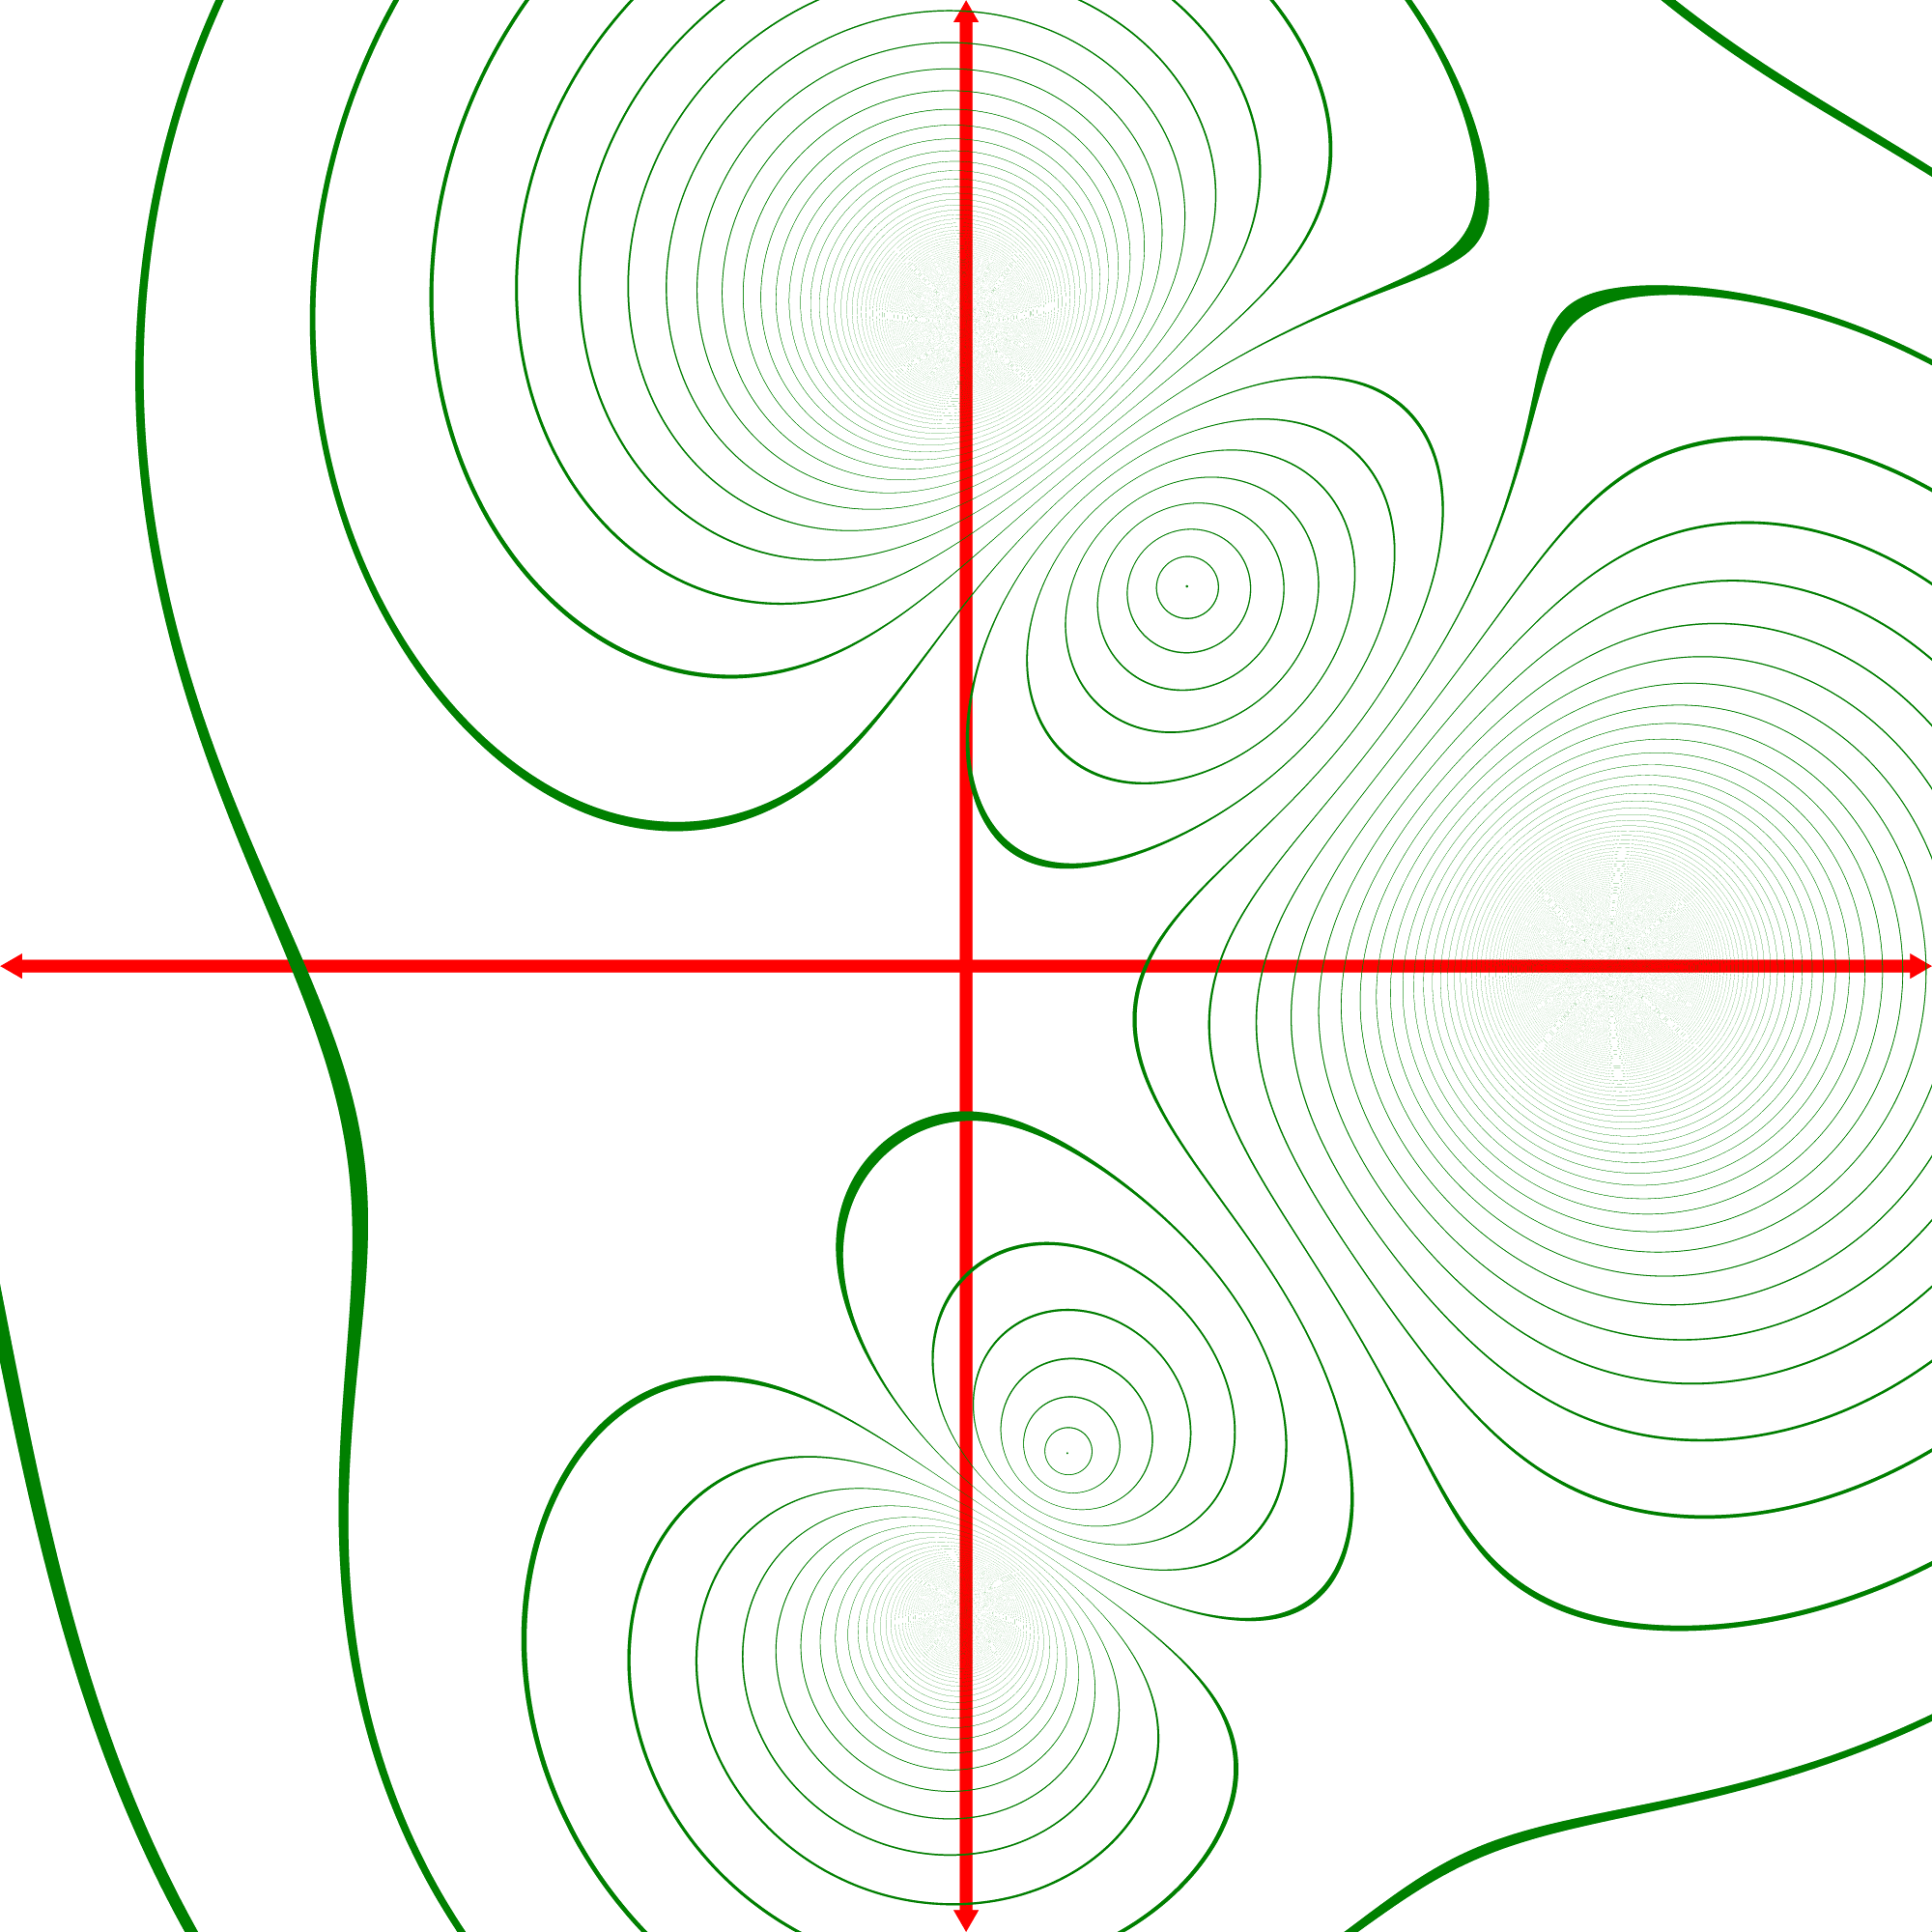
\includegraphics[scale=0.2]{images/charge_field.png}\\
        The green lines represent the values such that $\abs{\abs{f(z)} \mod{0.5}} <= 0.02$, or roughly the  0.5 increment level curves.
    \end{center}
\end{enumerate}
\end{document}
